\documentclass[a4paper]{article}
\usepackage[german]{babel}
\usepackage[utf8x]{inputenc}
\usepackage{amsmath}
\usepackage{amsfonts} 
% package for including graphics with figure-environment
\usepackage{graphicx}
\usepackage{hyperref}
\usepackage{float}
\usepackage{amssymb,stmaryrd}
% colors for hyperlinks
% colored borders (false) colored text (true)
\hypersetup{colorlinks=true,citecolor=black,filecolor=black,linkcolor=black,urlcolor=black}

% Commentbox package
\usepackage[most]{tcolorbox}
% Braket notation package
\usepackage{braket}

% package for bibliography
\usepackage[authoryear,round]{natbib}
% Commentbox package
\usepackage[most]{tcolorbox}
% package for header
\usepackage[automark,headsepline]{scrlayer-scrpage}
\pagestyle{scrheadings}
\ihead[]{Meyer, Springer, Kawamura, Heidenreich}
\ohead[]{\today}
\cfoot[]{\pagemark} 

\begin{document}
	\title{
	\begin{figure}[!ht]
		% \flushleft
			
\includegraphics[width=0.26\textwidth]{img/THlogoheader.pdf}
	\end{figure}
	\vspace{1cm}
	\Huge Here you can insert the title of \\ your seminar paper \\
	}
	
	\vspace{1cm}
	
	% if you are the only author, you might use the following
	% \author{Name of student}	
	
	% Insert here your name and correct mail address
	\author{\Large \href{mailto:ben_konrad.meyer@smail.th-koeln.de@smail.th-koeln.de}{Ben Konrad Meyer} \and \Large \href{mailto:mike.springer@smail.th-koeln.de}{Mike Springer} \and \Large \href{mailto:kai.kawamura@smail.th-koeln.de}{Kai Kawamura} \and \Large \href{mailto:karl_julian.heidenreich@smail.th-koeln.de}{Julian Heidenreich} \\
	\vspace{1cm}}
	
	% name of the course and module
	\date{
	\large Modul: Verteilte Systeme \\ 
	\vspace{0.8cm}
	\large Lecturer: Name of the lecturer \\
	\vspace{1cm}
	\today
	}

	\maketitle
	\setlength{\parindent}{0pt}

\vspace{2cm}
\begin{abstract}
This template can be used for seminar papers. For more tips and tricks regarding the use of figures, tables, quotations, references, footnotes, enumerations, etc. please download the Masterthesis template. 

\end{abstract}
	\newpage
	\tableofcontents
	\newpage
  
\section{Quantenbits} 
\label{sec:Quantenbits}
Ein Quantenbit, im Folgenden auch Qubit genannt, ist das Medium und die kleinste Einheit, auf dem in der Quanteninformatik gerechnet wird. Auf die genaue physische Realisierung wird in einem späteren Abschnitt der Quantenhardware eingegangen. Bis dahin reicht es das Quantenbit als eine Art Computer-Bit zu verstehen, das sich in einer sogenannten Superposition befindet. Im Zustand der Superposition kann es gleichzeitig den Wert ‚0‘ und ‚1‘ annehmen. Ein Quantenbit bleibt in dieser Superposition, bis es gemessen wird, woraufhin es diesen Zustand verliert und einen der Werte 0 und 1 annimmt. Die Wahrscheinlichkeit, mit der ein Quantenbit in den einen oder anderen Wert zerfällt, muss nicht gleichverteilt sein und kann beeinflusst werden. Dies macht Berechnungen auf Qbits erst möglich.
Mathematisch betrachtet, werden die Zustände ‚0‘ und ‚1‘ in der Quanteninformatik als Vektoren \verb|\(\binom{1}{0}\) \equiv| 0 und \verb|\(\binom{0}{1}\) \equiv| 1 dargestellt. Für die einfache Lesbarkeit werden diese Vektoren in der Quanteninformatik häufig in der sog. Ket-Darstellung beschrieben. 
Also \verb|\(\binom{1}{0}\)| \verb|\equiv| |0⟩ und \verb|\(\binom{0}{1}\)| \verb|\equiv| |1⟩. 
Um die Wahrscheinlichkeit zu beschreiben, welchen der beiden Werte ein Quantenbit nach der Messung annehmen wird, wird beiden Werten eine Amplitude \verb|\alpha| oder \verb|\beta| zugeordnet. Demnach wird ein Quantenbit in einer beliebigen Superposition als \verb|\alpha\cdot||0⟩+\verb|\beta\cdot||1⟩ dargestellt. \verb|\alpha| und \verb|\beta| sind komplexe Zahlen für die \verb|$\left|\alpha\right|^2+\left|\beta\right|^2=1$| gilt. 
Ein Qbit, das nach der Messung mit gleicher Wahrscheinlichkeit in einen der beiden Zustände 0 und 1 zerfällt, würde folglich als \frac{1}{\sqrt2}\bullet\left|0\right\rangle+\frac{1}{\sqrt2}\bullet\left|1\right\rangle dargestellt werden. Dabei gilt α = β = \frac{1}{\sqrt2} und erfüllt die Bedingung \left|\frac{1}{\sqrt2}\ \right|^2+\left|\frac{1}{\sqrt2}\ \right|^2=1 .
Ein Vektor \binom{\alpha}{\beta} wird als „Zustandsvektor“ bezeichnet und stellt den Zustand der Superposition eines Qubits dar. Die Bedingung \left|\alpha\right|^2+\left|\beta\right|^2=1 sorgt dafür, dass der Zustandsvektor immer ein Einheitsvektor ist. Dadurch kann jeder Zustand eines Qubits auf dem Einheitskreis eines zweidimensionalen Vektorsystems dargestellt werden. Somit kann ein Quantenbit unendlich viele Zustände haben, die auf einen definierten Bereich abgebildet werden können. 
Zum Zeitpunkt, als wir uns das Grundwissen erarbeitet haben, war uns nicht klar, weshalb α und β komplexe Zahlen sein sollten und warum sie „Amplituden“ und nicht „Wahrscheinlichkeiten“ oder Ähnliches genannt wurden. Wir gingen davon aus, dass wir früher oder später auf einen Use Case stoßen würden, in denen komplexe Zahlen und Amplituden wichtig werden würden. Dies war allerdings nur für die letzte Frage bedingt der Fall. Um kurz vorzugreifen: es gibt Algorithmen, in denen die Phase eines Zustandsvektors (also der Winkel des Zustandsvektors ausgehend vom Ursprung relativ zu einer der Achsen) eine wichtige Rolle spielt. Daher Amplituden? Kp.. Später kommt Sinus und Cosinus vor   

Wieso komplexe Zahlen? Weil Physik: siehe: https://www.cs.utep.edu/vladik/2023/tr23-44.pdf Man rechnet in Quanteninformatik eh nur mit reellen Zahlen.

Um mit Quantenbits rechnen zu können, muss man den Zustand eines Quantenbits verändern können. Wie dies physikalisch umgesetzt wird, wird später beschrieben. Aus mathematischer Sicht geschieht dies über unitäre 2x2 Matrizen. 
Eine Matrix A ist dann unitär, wenn ihre inverse Matrix A^{-1} gleich ihrer adjungierten Matrix A^\dag ist. Adjungiert ist eine Matrix A^\dag dann, wenn die Matrix A komplex konjugiert – also jedes Element der Matrix z_{ij}=\ a+ib zu z_{ij}^\ast\ =\ a\ – ib komplex konjugiert – und die Matrix dann transponiert wird. Für die Quanteninformatik reicht oft die Bedingung A^{-1}=A^T, da meistens mit α und β gerechnet wird, als seien sie reelle Zahlen. Durch diese Bedingung haben unitäre Matrizen die Eigenschaft, dass wenn sie zwei Mal mit einem Zustandsvektor verrechnet werden, der Zustandsvektor unverändert bleibt. Unitäre Transformationen sind also reversibel. Diese Bedingung ist notwendig, um die Länge der Zustandsvektoren beizubehalten.
Beispielhaft kann dies an einer Matrix B\ =\ \left(\begin{matrix}\frac{1}{2}&\frac{\sqrt3}{2}\\\frac{\sqrt3}{2}&-\frac{1}{2}\\\end{matrix}\right) demonstriert werden, die ein Qubit im Zustand|0⟩ in den Zustand \frac{1}{2}\left|\left.0\right\rangle\right.+\frac{\sqrt3}{2}\left|\left.1\right\rangle\right.  versetzt. Dies wird wie folgt berechnet:
B\left|\left.0\right\rangle\ =\ \right.\left(\begin{matrix}\frac{1}{2}&\frac{\sqrt3}{2}\\\frac{\sqrt3}{2}&-\frac{1}{2}\\\end{matrix}\right)\bullet\binom{1}{0}=\ \binom{\frac{1}{2}}{\frac{\sqrt3}{2}}
Daraus ergibt sich: \alpha\ =\ \frac{1}{2} und \beta\ =\ \frac{\sqrt3}{2}. Die Bedingung \left|\alpha\right|^2+\left|\beta\right|^2=1 trifft für beide Zustandsvektoren \binom{1}{0} und \binom{\frac{1}{2}}{\frac{\sqrt3}{2}} zu. Zudem ist B unitär, da B=\ B^T\ =\ B^{-1}, und daher eine zulässige Transformation.
Wenn man die Transformation B erneut an, ergibt sich folgendes:
B\binom{\frac{1}{2}}{\frac{\sqrt3}{2}}=\left(\begin{matrix}\frac{1}{2}&\frac{\sqrt3}{2}\\\frac{\sqrt3}{2}&-\frac{1}{2}\\\end{matrix}\right)\bullet\binom{\frac{1}{2}}{\frac{\sqrt3}{2}}=\ \binom{1}{0}.
Der Ursprungszustand ist mit der zweiten Anwendung der Transformation wieder hergestellt. Dies ist eine der Grundprinzipien der Quanteninformatik.
Hadamard-Matrix
Eine unitäre Transformation, die im Laufe unseres Lernprozesses immer wieder vorgekommen ist, ist die sog. Hadamard-Matrix H=\left(\begin{matrix}\frac{1}{\sqrt2}&\frac{1}{\sqrt2}\\\frac{1}{\sqrt2}&-\frac{1}{\sqrt2}\\\end{matrix}\right). Multipliziert mit dem Zustand |0⟩ transformiert sie ihn in den Zustand \frac{1}{\sqrt2}(\left|\left.0\right\rangle+\right.\left|\left.1\right\rangle)\right. und mit |1⟩ transformiert sie ihn in den Zustand \frac{1}{\sqrt2}(\left|\left.0\right\rangle-\right.\left|\left.1\right\rangle)\right.. Beide Folgezustände haben die gleiche Wahrscheinlichkeit bei der Messung in einen der Zustände |0⟩ oder |1⟩ zu zerfallen.
Damit ließe sich beispielsweise ein Münzwurf simulieren. Der Schaltkreis eines Münzwurfs sieht folgendermaßen aus: [hier Bild vom Münzwurfschaltkreis einfügen] Schaltkreise eigenen sich dafür Quantenalgorithmen anschaulich darzustellen. Auf sie wird später genauer eingegangen.
Zuerst wird ein Quantenbit in den Zustand |0⟩ gebracht. (Man könnte es auch in den Zustand |1⟩ bringen. Das ist für diesen Algorithmus unwichtig.) Danach wendet man die Hadamard-Transformation darauf an, um das Quantenbit in eine Superposition zu bringen, in der |0⟩ und |1⟩ mit gleicher Wahrscheinlichkeit vorkommen. Anschließend wird gemessen und die Superposition zerfällt zufällig in einen der Zustände |0⟩ oder |1⟩.
Formal beschrieben sieht der Algorithmus so aus:
	\left|\left.x\right\rangle\right.\ \gets\ \left|\left.0\right\rangle\right.\ 
	\left|\left.x\right\rangle\right.\ \gets\ H\left|\left.x\right\rangle\right.
	Miss\left|\left.x\right\rangle\right.
„|x⟩“ ist dabei die Bezeichnung des Quantenbits auf dem gerechnet wird.
Mit diesem Algorithmus ist möglich echte Zufallszahlen zu generieren, da es physikalisch unmöglich ist vorauszusagen, in welchen Zustand die Superposition zerfallen wird. Im Gegensatz zu einem echten Münzwurf, bei dem man das Wurfergebnis theoretisch berechnen könnte, wenn man sämtliche Variablen, wie z.B. Wurfhöhe, Drehmoment der Münze, Luftwiederstand, ect. kennen würde. Oder im Gegensatz zu einem herkömmlichen Computer, der nur Pseudozufallszahlen generieren kann. 
Quantenregister
Ein Quantenregister ist eine Aneinanderreihung mehrerer voneinander unabhängiger Quantenbits. Diese werden benötigt, um Quantenschaltkreise zu realisieren, damit auf ihnen logische Operationen durchgeführt werden können. 
Der Zustand eines Quantenregisters der Länge m wird als m-faches Tensorprodukt aller Zustände der einzelnen Quantenbits des Registers dargestellt. Ein Quantenregister R mit 2 Qubits \left|\left.x_0\right\rangle\ \right.und \left|\left.x_1\right\rangle\ \right.in beispielsweise den Basiszuständen \left|\left.x_0\right\rangle\ \right.=\binom{0}{1} und \left|\left.x_1\right\rangle\ \right.=\binom{1}{0} befindet sich im Zustand:
R\ =\ \left|\left.x_0\right\rangle\ \right.\otimes\left|\left.x_1\right\rangle\ \right.=\binom{0}{1}\otimes\binom{1}{0}=\left(\begin{matrix}0\\\begin{matrix}0\\\begin{matrix}1\\0\\\end{matrix}\\\end{matrix}\\\end{matrix}\right)
Alternativ würde man R =|1⟩ ⊗ |0⟩ = |10⟩ schreiben. Manchmal werden die Basiszustände zur Übersichtlichkeit auch in dezimalform dargestellt. |10⟩ wäre demnach |2⟩. 
Wie auch die einzelnen Qubits, kann sich das gesamte Quantenregister in einer Superposition befinden. Sind die Qubits aus dem obigen Beispiel in den Zuständen 
\left|\left.x_0\right\rangle\right.=\beta_0\left|\left.0\right\rangle\ \right.+\beta_1\left|\left.1\right\rangle\ \right.und \left|\left.x_1\right\rangle\right.=\gamma_0\left|\left.0\right\rangle\ \right.+\gamma_1\left|\left.1\right\rangle\ \right.
ist der Zustand des Quantenregisters 
R=\ \left|\left.x_0\right\rangle\right.\left|\left.x_1\right\rangle\right.=\left(\beta_0\left|\left.0\right\rangle\ \right.+\beta_1\left|\left.1\right\rangle\ \right.\right)\bullet(\gamma_0\left|\left.0\right\rangle\ \right.+\gamma_1\left|\left.1\right\rangle\ \right.)\ =\beta_0\gamma_0\left|\left.0\right\rangle\ \right.\left|\left.0\right\rangle\ \right.+\beta_0\gamma_1\left|\left.0\right\rangle\ \left|\left.1\right\rangle\ \right.\right.+\ \beta_1\gamma_0\left|\left.1\right\rangle\ \right.\left|\left.0\right\rangle\ \right.+\beta_1\gamma_1\left|\left.1\right\rangle\ \right.\left|\left.1\right\rangle\ \right.
Substituiert man \beta_i\gamma_j=\alpha_{ij} ergibt sich der Zustand
R=\alpha_{00}\left|\left.0\right\rangle\ \right.\left|\left.0\right\rangle\ \right.+\alpha_{01}\left|\left.0\right\rangle\ \left|\left.1\right\rangle\ \right.\right.+\ \alpha_{10}\left|\left.1\right\rangle\ \right.\left|\left.0\right\rangle\ \right.+\alpha_{11}\left|\left.1\right\rangle\ \right.\left|\left.1\right\rangle\ \right.
Und kann als
R=\alpha_{00}\left|\left.00\right\rangle\ \right.+\alpha_{01}\left|\left.01\right\rangle\right.+\ \alpha_{10}\left|\left.10\right\rangle\ \right.+\alpha_{11}\left|\left.11\right\rangle\ \right.
Oder
R=\alpha_0\left|\left.0\right\rangle\ \right.+\alpha_1\left|\left.1\right\rangle\right.+\ \alpha_2\left|\left.2\right\rangle\ \right.+\alpha_3\left|\left.3\right\rangle\ \right.
Geschrieben werden.
Da aus \left|\beta_0\right|^2+\left|\beta_1\right|^2=1 und \left|\gamma_0\right|^2+\left|\gamma_1\right|^2=1 sich \left|\alpha_{00}\right|^2+\left|\alpha_{01}\right|^2+\left|\alpha_{10}\right|^2+\left|\alpha_{11}\right|^2=1 ergibt, bildet α die Amplitude für den jeweiligen Zustand \left|\left.00\right\rangle\right.,\left|\left.01\right\rangle\right.,\left|\left.10\right\rangle\right.\ und\ \left|\left.11\right\rangle\right.. 
Allgemeiner gefasst befindet sich ein Quantenregister R der Länge n im Zustand 
R=\sum_{i=0}^{2^n-1}{\alpha_i\left|\left.i\right\rangle\right.}.
Für den die Bedingung
\sum_{i=0}^{2^n-1}\left|\alpha_i\right|^2=1
Gilt. Dabei entspricht i=0,...,2^n-1 der Dezimaldarstellung der Bits im Quantenregister und \left|\alpha_i\right|^2 der Wahrscheinlichkeit, dass sich das Register nach einer Messung im jeweiligen Zustand \left|\left.i\right\rangle\right. befindet.
Es ist möglich Transformationen nicht nur auf einzelnen Quantenbits durchzuführen, sondern auch auf ganze Register. Um eine Transformation auf einem Register eine Transformation durchzuführen, muss zuerst ein möglicherweise mehrfaches Tensorprodukt der Transformationsmatrix mit sich selbst berechnet werden. Da ein Tensorprodukt nur zwischen Matrizen derselben Größe berechnet werden kann, ist es nur möglich Transformationen auf 2^n langen Registern durchzuführen. 
Wir vermuten, dass wenn man eine Transformation auf ein Register der Länge m anwenden möchte, wobei m nicht in der Menge ist, die mit 2^n abgebildet werden kann, man das Register in zwei Unterregister aufteilen kann. Und die Transformation auf die Unterregister ausführt (Länge 2^max(n) < m und Länge Rest..) Da Rechenschritte physikalisch nur lokal durchgeführt werden können (s.31) scheint es für uns keinen Unterschied zu machen, auf wie vielen Qubits eine Transformation mathematisch durchgeführt wird.
Die Transformationen A_1,\ldots,A_{2^n} auf die Bits \left|\left.x_1\right\rangle\right.,\ldots,\left|\left.x_{2^n}\right\rangle\right. mit jeweils A_i\ auf \left|\left.x_i\right\rangle\right. entsprechen also der Transformation A_1\otimes,\ ...\ ,\otimes A_{2^n}\ auf das Register \left|\left.x_1,...,x_{2^n}\right\rangle\right..
Möchte man die Hadamard-Transformation H auf ein Register R = |00⟩ anwenden, müsste man zuerst die Hadamard-Transformation auf Registerebene 
H\otimes H\ =\ H_2=\ \frac{1}{\sqrt2}\left(\begin{matrix}H&H\\H&-H\\\end{matrix}\right)=\frac{1}{2}\left(\begin{matrix}\begin{matrix}1&1\\1&-1\\\end{matrix}&\begin{matrix}1&1\\1&-1\\\end{matrix}\\\begin{matrix}1&1\\1&-1\\\end{matrix}&\begin{matrix}-1&-1\\-1&1\\\end{matrix}\\\end{matrix}\right)
bilden. Daraus ergibt sich
H_2R\ =\frac{1}{2}\left(\begin{matrix}\begin{matrix}1&1\\1&-1\\\end{matrix}&\begin{matrix}1&1\\1&-1\\\end{matrix}\\\begin{matrix}1&1\\1&-1\\\end{matrix}&\begin{matrix}-1&-1\\-1&1\\\end{matrix}\\\end{matrix}\right)\binom{\begin{matrix}1\\0\\\end{matrix}}{\begin{matrix}0\\0\\\end{matrix}}=\binom{\begin{matrix}\frac{1}{2}\\\frac{1}{2}\\\end{matrix}}{\begin{matrix}\frac{1}{2}\\\frac{1}{2}\\\end{matrix}}\ 
Beziehungsweise \frac{1}{2}\left(\left|\left.00\right\rangle\right.+\left|\left.01\right\rangle\right.+\left|\left.10\right\rangle\right.+\left|\left.11\right\rangle\right.\right) oder \frac{1}{2}\left(\left|\left.0\right\rangle\right.+\left|\left.1\right\rangle\right.+\left|\left.2\right\rangle\right.+\left|\left.3\right\rangle\right.\right).
Dabei bleibt die Bedingung 
\sum_{i=0}^{2^n-1}\left|\alpha_i\right|^2=1
 Mit n = 2 und \alpha_i\ =\ \frac{1}{2}\ \forall\ i erfüllt. Die Wahrscheinlichkeit, dass jeder Basiszustand nach der Messung auftritt, ist gleichverteilt. Diese Berechnung kann genutzt werden, um echte zufallszahlen zwischen 0 und 3 zu generieren. Formal beschrieben sieht der Algorithmus aus, wie folgt:
	R=\left|\left.x_1x_0\right\rangle\right.\gets\left|\left.00\right\rangle\right.
	R=H_2R
	Miss R
Dieser Algorithmus kann auf eine beliebige Registergröße 2^n erweitert werden. 
Allerdings ist das Rechnen auf Registerebene bisher nur mathematisch sinnvoll. Tatsächlich werden sämtliche Rechenschritte in lokalen unitären Transformationen durchgeführt. „Lokal“ heißt in diesem Fall, dass maximal drei Qubits an der Berechnung beteiligt sind, da es physikalisch einfacher ist Transformationen auf drei Bits auszuführen als auf 2^n mit beliebig hohen n. Zudem sind mindestens drei Bit notwendig, um klassische Rechenverfahren in Quantenalgorithmen zu überführen. Dies wird später deutlich.
In den beiden Münzwurfbeispielen wurde die Hadamard-Transformation nur auf Quantenbits oder -register angewandt, bei denen sich alle Bits im Zustand |0⟩ befunden haben. Ein n langes Quantenregister R, dessen Bits sich alle im Zustand |0⟩ befunden haben und auf das die Hadamard-Transformation angewandt wurde, kann wie folgt dargestellt werden:
R=\frac{1}{\sqrt{2^n}}\sum_{i=0}^{2^n-1}\left|\left.i\right\rangle\right.
Diese Darstellung reicht allerdings nicht aus, um Quantenregister abzubilden, dessen Quantenbits sich vor der Hadamard-Transformation teilweise im Zustand |1⟩ befunden haben. Wendet man die Hadamard-Transformation auf ein Register |xy⟩ an, das sich im Zustand |01⟩ befindet, sähe das Quantenregister vor dem Ausmultiplizieren wie folgt aus:
\left|\left.01\right\rangle\right.{\buildrelH_2\frac\rightarrow}\frac{1}{\sqrt2}(\left|\left.0\right\rangle\right.+\left|\left.1\right\rangle\right.)\bullet\frac{1}{\sqrt2}(\left|\left.0\right\rangle\right.-\left|\left.1\right\rangle\right.).
Man kann an dieser Stelle die Information, ob sich die jeweiligen Quantenbits vorher im Zustand |0⟩ oder |1⟩ befunden haben, in das Vorzeichen ziehen:
\left|\left.xy\right\rangle\right.{\buildrelH_2\frac\rightarrow}\frac{1}{\sqrt2}(\left|\left.0\right\rangle\right.+{(-1)}^x\left|\left.1\right\rangle\right.)\bullet\frac{1}{\sqrt2}(\left|\left.0\right\rangle\right.+{(-1)}^y\left|\left.1\right\rangle\right.).
Ausmultipliziert ergibt dies: 
\frac{1}{2}\left(\left|\left.00\right\rangle\right.+\left(-1\right)^x\left|\left.01\right\rangle+\left(-1\right)^y\left|\left.10\right\rangle\right.+\left(-1\right)^{x\oplusy}\left|\left.11\right\rangle\right.\right.\right).\bigmAllgemeiner gefasst:
\frac{1}{2}\left(\left(-1\right)^{\left(0,0\right)\oplus z}\left|\left.00\right\rangle\right.+\left(-1\right)^{\left(0,1\right)\oplus z}\left|\left.01\right\rangle+\left(-1\right)^{\left(1,0\right)\oplus z}\left|\left.10\right\rangle\right.+\left(-1\right)^{\left(1,1\right)\oplus z}\left|\left.11\right\rangle\right.\right.\right),
mit z={(x,y)}^T.
Muss zugeben, den Sinn von diesem Ausmultiplizieren habe ich am Anfang nicht verstanden. Wahrscheinlich wird das bei komplexeren Algorithmen erst relevant.
Anhand der letzten Darstellung kann man ein Quantenregister der Lände n im Zustand
x\in{{0,1}}^n, auf das die Hadamard-Transformation angewandt wurde, wie folgt darstellen:
H_n\left|\left.x\right\rangle\right.=\frac{1}{\sqrt{2^n}}\sum_{y\in{0,1}^n}\left(-1\right)^{x\bullety}\left|\left.y\right\rangle\right..
Dabei ist x⋅y das Skalarprodukt \oplus_{i=1}^nx_iy_i der Vektoren x,y\in{{0,1}}^n. 
Auch die Hadamard-Transformation ist reversibel. Nehmen wir das vorherige Beispiel:
\left|\left.01\right\rangle\right.{\buildrelH_2\frac\rightarrow}\frac{1}{\sqrt2}(\left|\left.0\right\rangle\right.+\left|\left.1\right\rangle\right.)\bullet\frac{1}{\sqrt2}(\left|\left.0\right\rangle\right.-\left|\left.1\right\rangle\right.).
Wendet man die Hadamard-Transformation erneut an, ergibt sich:
\frac{1}{\sqrt2}\left(\left|\left.0\right\rangle\right.+\left|\left.1\right\rangle\right.\right)\bullet\frac{1}{\sqrt2}\left(\left|\left.0\right\rangle\right.-\left|\left.1\right\rangle\right.\right)\bigm{\buildrelH_2\frac\rightarrow}\frac{1}{\sqrt2}\left(\frac{1}{\sqrt2}\left(\left|\left.0\right\rangle\right.+\left|\left.1\right\rangle\right.\right)+\frac{1}{\sqrt2}\left(\left|\left.0\right\rangle\right.-\left|\left.1\right\rangle\right.\right)\right)\bullet\frac{1}{\sqrt2}\left(\frac{1}{\sqrt2}\left(\left|\left.0\right\rangle\right.+\left|\left.1\right\rangle\right.\right)-\frac{1}{\sqrt2}\left(\left|\left.0\right\rangle\right.-\left|\left.1\right\rangle\right.\right)\right)\bigm=\frac{1}{\sqrt2}\left(\frac{1}{\sqrt2}\left(\left|\left.0\right\rangle\right.+\left|\left.0\right\rangle\right.\right)\right)\bullet\frac{1}{\sqrt2}\left(\frac{1}{\sqrt2}\left(\left|\left.1\right\rangle\right.+\left|\left.1\right\rangle\right.\right)\right)\bigm=\frac{1}{2}\left(\left|\left.0\right\rangle\right.+\left|\left.0\right\rangle\right.\right)\bullet\frac{1}{2}\left(\left|\left.1\right\rangle\right.+\left|\left.1\right\rangle\right.\right)\ =\frac{1}{4}\left(\left|\left.01\right\rangle\right.+\left|\left.01\right\rangle\right.+\left|\left.01\right\rangle\right.+\left|\left.01\right\rangle\right.\right)=\left|\left.01\right\rangle\right..
Die Reversibilität der Hadamard-Transformation ist für komplexere Algorithmen von Bedeutung. Bevor auf diese und deren Darstellung in Form von Quantenschaltkreisen eingegangen werden kann, muss vorher noch auf den Vorgang der Messung eingegangen werden.
Messen
Die Messung „Miss|x⟩“ die einzige Transformation in der Quanteninformatik, die nicht reversibel / unitär ist. Beim Messen verliert das Quantenbit die Superposition und fällt zufällig, je nach Wahrscheinlichkeitsverteilung in einen der Zustände |0⟩ oder |1⟩. Aus diesen Zuständen ist nicht zu errechnen in welchem Zustand sich das Quantenbit vor der Messung befunden hat. Daher ist die Messung meist der letzte Schritt, den man für ein Quantenbit innerhalb eines Algorithmus durchführt. Das bedeutet allerdings nicht, dass die Messung aller Quantenbits immer am Ende eines Algorithmus geschehen muss. Es gibt Algorithmen in denen man zum Beispiel das Zwischenergebnis eines Quantenbits misst und anhand dieser Messung bestimmt, welche folgenden Transformationen für andere Quantenbits durchgeführt werden müssen. 

\end{document}
\section{Der Kontrast zwischen Klassischen und Quantencomputern}

- Qubit vs Klassisches Bit

- Umkehrbare Operationen in QC

- Alle KC Operationen in QC möglich, aber teilweise komplexer

- QC kann Operationen machen, die der KC nicht kann (größtenteils Zufallselemente)

- Zwei Beispiele folgen, die das verdeutlichen

\subsection{No Cloning Theorem}

- Proof by Contradiction (Umkehrbare Operationen)

- Macht Klassische Error Correction unmöglich

\subsection{Verschränkte Teleportation}

- Braucht Setup (verschränktes Qubit teilen)

- überträgt einen Quantenzustand

- - Zustand am Ursprung wird zerstört (no cloning theorem)

\section{Quantenhardware}
\label{sec:quantenhardware}

Die Realisierung eines Quantencomputers ist durch hohe technische herausforderungen geprägt. Um die besonderen Eigenschaften der Qubits eines Quantencomputers, wie Superposition und Verschränkung, nutzen zu können, müssen sie durch externe Einflüsse geschützt werden und die Dekoheränz minimiert werden.
Äußere Einflüsse wie Temperaturschwankungen, elektromagnetische Felder oder Strahlung aller Art können die Qubits beeinflussen. Aus diesem Grund werden Quantencomputer bei extrem niedrigen Temperaturen und in einem Vakuum betrieben.\\

Außerdem ist nicht nur die Herstellung der Qubits eine Herausforderung, sondern auch die Steuerung, Auslesung und Korrektheit von physikalischen Qubits.

\subsection{Dekohärenz}
\label{sub:dekohaerenz}
Dekoheränz ist ein zentrales Konzept, welches wichtig in der Entwicklung von Quantencomputern ist. Der Prozess der Dekoheränz beschreibt den Verlust der koheränten Quanteneigentschaften eines Qubits durch Wechselwirkung mit der Umgebung.
Diese Veränderung führt zu einem Übergang von quantenmechanischem Verhalten zu einem klassischem Verhalten von Bits.\\

In der Quantenmechanik können Systeme in Überlagerungszuständen existieren, wobei mehrere Zustände gleichzeitig eingenommen werden können. Diese Eigenschaft erklärt auch das Phänomen der Quanteninterferenz.
Äußere Einflüsse durch die Umgebung kann eine Verschränkung von Qubits zerstören. Dies führt dazu, dass die Phasenbeziehungen zwischen den Qubits beeinflusst oder gar aufgehoben werden.
Folgernd verliert das System die Interferenzeffekte und verhält sich zunehmend klassischer. Diese Zeit nennt man Dekoheränzzeit.\\

Die \textbf{Dekoheränzzeit} ($T_2$) eines Qubits misst die Länge der Zeit, in der er in der Lage bleibt kohärent zu bleiben, welcher danach von äußeren Einflüssen zerstört wird.
Neben $T_2$ wird auch häufig die \textbf{Relaxationszeit} ($T_1$) gemessen, welche angibt, wie lange ein Qbit im angeregten Zustand bleibt, bevor es auf sein Grundzustand zurückfällt.
In der Realität ist die Dekoheränzzeit jedoch in den meisten Fällen kürzer als die Relaxationszeit.\\

\textbf{Berechnung der Dekoheränzzeit}\\
Durch eine Messung der zeitlichen Abnahme der Koheränz eines beispielhaften Qubits kann die Dekoheränzzeit eines Systems festgelegt werden.
Bei einem Quantencomputer, der auf dem Spin eines Teilchen beruht, kann dies durch die \textbf{Spin-Echo-Methode} gemessen werden.
Quantencomputer, die auf anderen Qubits basieren, haben equivalente Methoden um die Kohärenz zu messen.\\

Das einfachste Modell zur Beschreibung der Dekoheränzzeit ist die \textbf{Exponentielle Abnahme der Kohärenz}

\begin{equation}
    C(t) = C(0)*e^{-t/T_2}
\end{equation}

Dabei ist:\\
$C(t)$ Die Kohärenz des Qubits zum Zeitpunkt t\\
$C(0)$ Die initiale Koheränz\\
$T_2$ Die Dekoheränzzeit\\

Indem man den Kohärenzverlust experimentell misst und die Werte in eine exponentielle Abklingfunktion einpasst, erhält man $T_2$\\

\begin{tcolorbox}[title=Kommentar,
    title filled=false,
    colback=cyan!5!white,
    colframe=cyan!75!black]
    Die \textbf{Dekoheränzzeit} kann auch durch genauere jedoch auch deutlich kompliziertere weise errechnet werden.
    Bekannte Methoden hierfür wären zum Beispiel die Spektrale Analyse, Dynamische Entkopplung, Hahn-Echo und Ramsey-Interferometrie.
    Außerdem wird duch das häufige messen der Dekoheränzzeit diese indirekt verlänger. Diesen Effekt nennt man Quanten-Zeno-Effekt.\\
    Zuletzt muss auch die Lindblad-Gleichung genannt werden welche den Zeitverlauf der Dichtematrix in einem Offenen Quantensystem beschreibt.
    \begin{equation}
        \frac{dp}{dt} = -i[H,p]+\sum_i(L_ipL^\dagger_i-\frac{1}{2}\{L^\dagger_i L_i,p\})
    \end{equation}
    Diese Themen sprengen jedoch den Rahmen dieser Arbeit in Richtung Physik und werden deswegen nicht weiter behandelt.
\end{tcolorbox}

\subsection{Universelle Quantencomputer}
\label{sub:universelle_quantencomputer}
Universelle Quantencomputer beruhen grundlegend auf einem Gatter Modell, wie bereits in diesem Artikel beschrieben. Folgend sind drei der meist erforschten
Methoden, welche dieses Modell physikalisch umsetzen.\\

Ein prominentes Beispiel für die Umsetzung eines universellen Quantencomputers ist der \textbf{Sycamore Chip}, welcher auf supraleitenden Qubits basiert.
Dieser Chip ist in einem Gatter angeordnet für die Kommunikation zwischen Qubits und die durchführung von Quantenoperationen.\\

\begin{figure}[H]
    \centering
    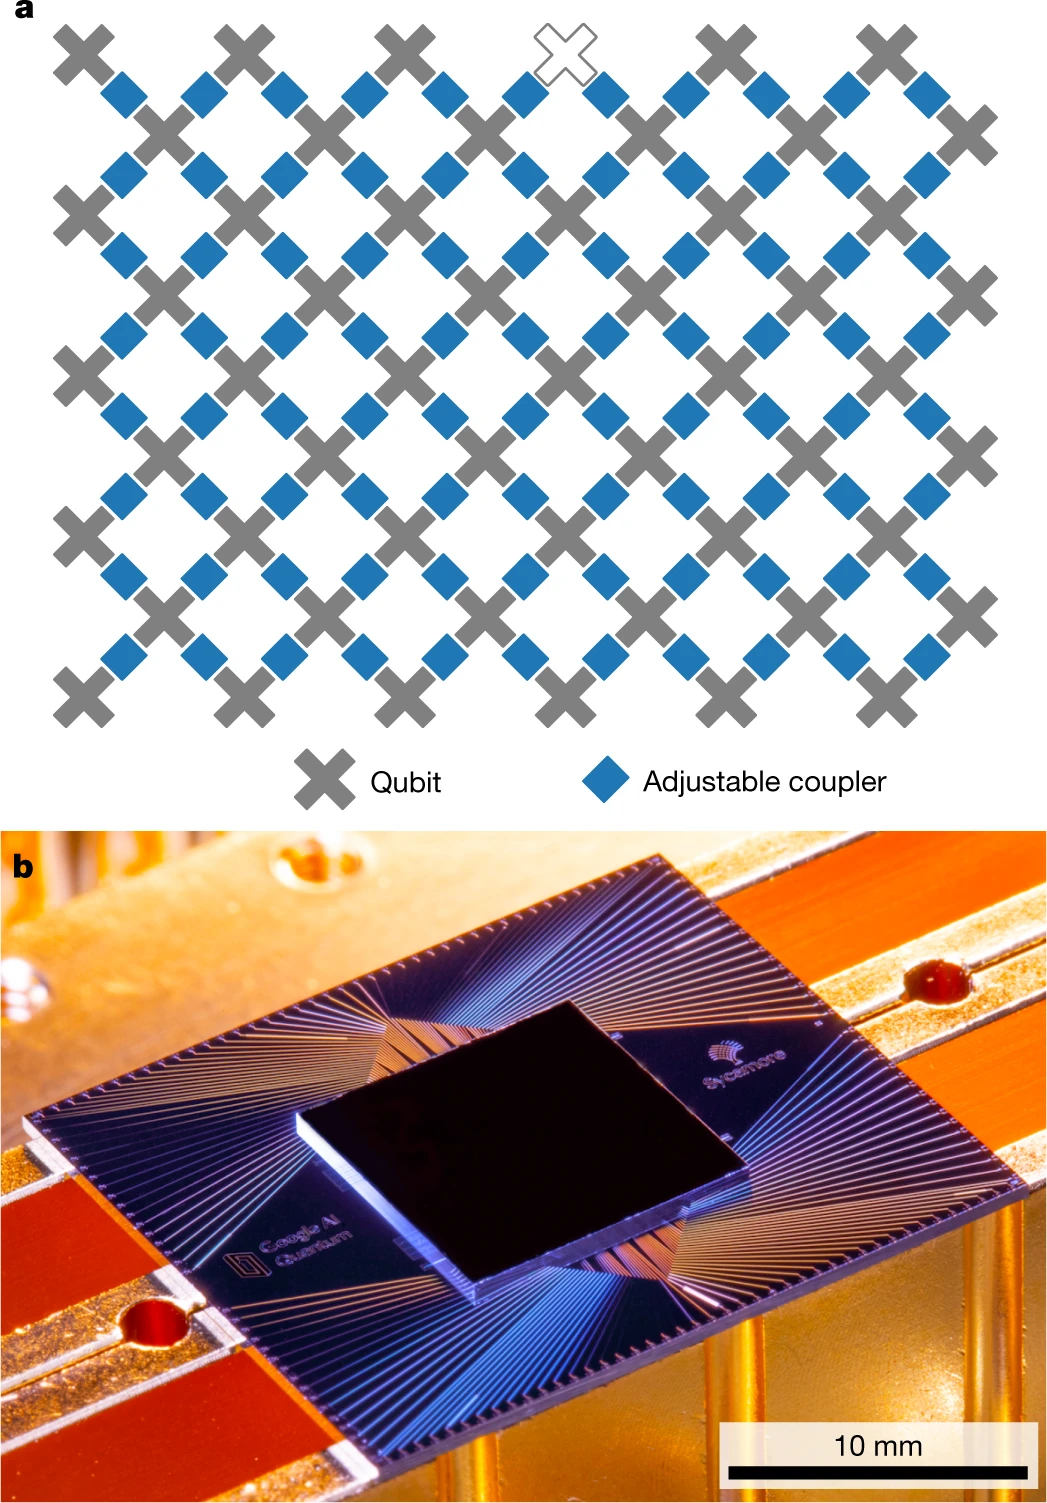
\includegraphics[width=0.7\linewidth]{img/SycamoreChip.png}
    \caption{Sycamore Chip von Google}
    \label{fig:Sycamore}
\end{figure}

\subsubsection{Supraleitende Qubits}
\label{subsub:superleiter}
Quantencomputer mit Supraleitern funktionieren mit elektrischen Schaltkreisen, die bei Temperaturen nahe dem absoluten Nullpunkt betrieben werden. Solche Temperaturen sind nötig,
um die supraleitende Eigenschaft aufrecht zu erhalten.\\

Zwei häufig benutze Qubit-Typen dieser elektrischen Schaltkreise sind:\\
\textbf{Transmon-Qubits}, basiert auf der Ladung des Energieniveaus, welche durch eine Josephson-Junktion kontrolliert wird.\\
\textbf{Flux-Qubits} werden auch durch Josephson-Junktions kontrolliert, beruhen jedoch auf dem magnetischen Fluss in der Schleife.\\

Beide Ansätze basieren auf dem \textbf{Josephson-Effekt}, welcher auftritt, wenn ein supraleitender Strom durch eine dünne Isolierschicht zwischen zwei Supraleitern fließt.\\
Dieser Effekt hat zur Folge, dass eine nichtlineare Spannung-Stom-Beziehung entsteht und für die Manipulation von Qubits genutzt wird.\\

\begin{figure}[H]
    \centering
    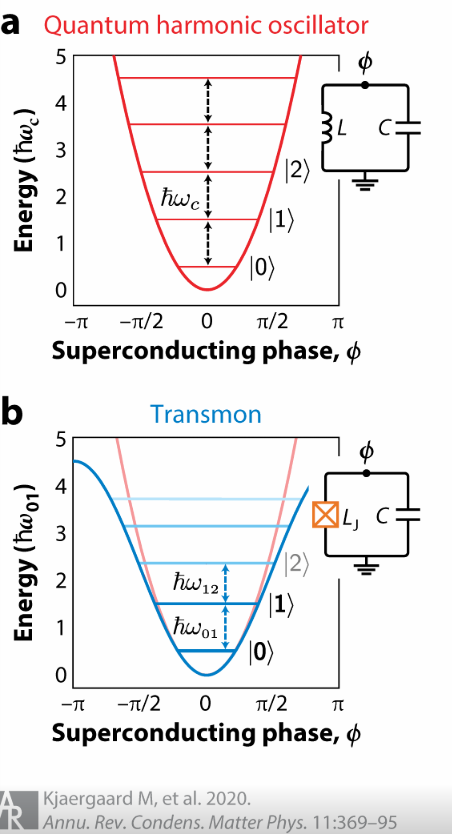
\includegraphics[width=0.75\linewidth]{img/JJ.png}
    \caption{Josephson-Effekt mit einem Josephson Junktion}
    \label{fig:Josephson-junktion}
\end{figure}

In der vorliegenden Abbildung wird der Unterschied zwischen einer harmonischen Quantenschwankung (a) und der nichtlinearen Schwankung des Energie Niveaus der Josephson Junktion (b) abgebildet.\\

Der Phasenunterschied bei der harmonischen Oscellation, gekennzeichnet als $\hbar\omega_c$, ist identisch. Auf der Abbildung ist zu sehen, dass das Energieniveau der Phasen zwischen $\ket{0} \leftrightarrow \ket{1}$
und $\ket{1} \leftrightarrow \ket{2}$ identisch ist und dadurch nicht unterschieden werden kann zwischen welcher Phase gewechselt wurde.\\

Mit einer Josephson Junktion kann jedoch eine nichtlineare Schwankung des Energieniveaus erreicht werden, die auf der Abbildung als orangenes $\boxtimes$ gekennzeichnet ist (b).
Durch diese nichtlineare Schwankung ist das Energie Niveau zwischen den Phasen $\ket{0} \leftrightarrow \ket{1}$ und $\ket{1} \leftrightarrow \ket{2}$ unterschiedlich groß und kann somit unterschieden werden.
Der als $\hbar\omega_{01}$ gekennzeichnete Energieunterschied ist unser Qubit\\

\textbf{Steuerung und Auslesung}\\
Die Steuerung der Josephson-Junktion erfolgt durch Mikrowellenpulse, welche die Energie des Qubits verändern. Die Auslesung erfolgt durch eine Mikrowellenresonanz um die Energie des Qubits zu messen.\\

\subsubsection{Quantenpunkte}
\label{subsub:quantenpunkte}
Quantencomputer basierend auf Quantenpunkten, auch Quantum-Dot genannt, nutzen winzige Halbleiterstrukturen um Qubits zu realisieren.
Quantum-Dots sind künstlich erzeugte Nano-Partikel, in denen Elektronen in drei Dimensionen eingeschlossen sind, was zu quantisierten Einergiezuständen führt.\\

Die Größe eines Quantum-Dots ist typischerweise 2-10 Nanometer und es schließt eine kleine Anzahl oder ein einzelnes Elektron ein.
Für die Fertigung werden oftmals Galliumarsenid (GaAs) oder Silizium (Si) verwendet. Der physikalische Einschluss der Elektronen schränkt ihre
Bewegung stark ein, wodurch ein quantisiertes Energieniveau entsteht. Dies ähnelt dem Energieniveaus eines Atoms, weswegen Quantum-Dots auch als künstliche Atome bezeichnet werden.\\

Die Zustände der Qubits werden durch die Eigenschaften einzelner Elektronen in den Quantum Dots definiert. Es gibt zwei Hauptansätze zur Realisierung von Qubits mit Quantum Dots.\\

\textbf{Ladungs-Qubits}\\
Der Ladungszustand eine Quantum Dots kann als Qubit verwendet werden. Die Ladung eines Elektrons kann entweder 0 oder 1 sein, was als $\ket{0}$ und $\ket{1}$ interpretiert wird.
Für eine Messung wird der Ladungszustand mit einer Kapazitätsmessung der Tunnelströme ermittelt.
Für die Manipulation des Qubits werden elektrische Felder verwendet, um die Elektronen in den Quantum Dots zu bewegen.\\

Diese Methode ist durch die Ladungsquantisierung sehr genau, jedoch auch sehr empfindlich gegenüber Störungen durch die Umgebung.\\

\textbf{Spin-Qubits}\\
Die Spin-Eigenschaften von Elektronen in Quantum Dots können auch als Qubit verwendet werden. Hierbei sind die beiden Spinrichtungen($\uparrow$ für Spin-Up und $\downarrow$ für Spin-Down)
dieser beiden Spinrichtungen entsprechen den Zuständen $\ket{0}$ und $\ket{1}$. Und die Kombination aus beiden Zuständen ergibt eine Superposition.\\

\begin{figure}[H]
    \centering
    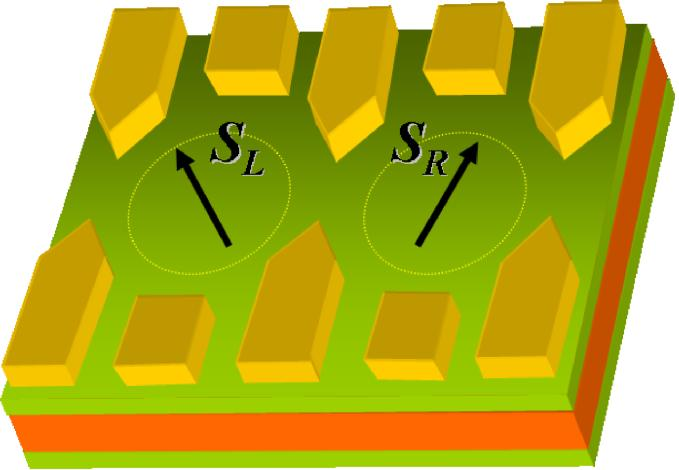
\includegraphics[width=0.75\linewidth]{img/QD.png}
    \caption{Ein doppel Quantum-Dot Qubit}
    \label{fig:double-Quantum-Dot}
\end{figure}

In der Abbildung ist ein Doppel Quantum-Dot Qubit dargestellt. Sowohl in $S_L$ als auch $S_R$ befinden sich Elektornen. Beide können seperat voneinander, sowohl im Spin als auch Ladung, manipuliert werden.
Durch die physikalische Nähe der beiden Quantum-Dots können durch Tunnelkopplung und Austauschwechselwirkung die beiden Qubits miteinander verschränkt werden.\\

Die Umsetzung dieser Methode beschränkt sich hauptsächlich auf die Spin-Variante. Der Grund dafür ist, dass durch die hohe Ladungsanforderung der Ladungsvariante die Qubits sehr empfindlich gegenüber Störungen sind.
Außerdem sind die Nachteile der Spin-Variante gegenüber der Ladungsvariante nicht so gravierend.\\
Jedoch sind die größten Herausforderungen die Herstellung der Halbleiterstrukturen und die Kontrolle der Elektronen in den Quantum-Dots.
Damit ist der größte Vorteil, die hohe Skalierbarkeit, auch der größte Nachteil, da die Herstellung und Kontrolle von vielen Quantum-Dots sehr aufwendig und schwierig ist.\\

\subsubsection{Topologische Quantencomputer}
\label{subsub:topologische_quantencomputer}
Der Ansatz von topologischen Quantencomputern ist völlig anders als die bisher genannten. Im Gegensatz zu verher erläuterten Quantencomputern, welche auf Eigenschaften einzelner Elektronen oder Energieniveaus basieren, basieren topologische Quantencomputer auf topologischen Eigenschaften von Materie.\\
Diese Methode soll das Problem der Dekoheränz minimieren, indem sie Qubits aus Majorana-Partikeln aufbauen.\\

\textbf{Topologie in der Physik}\\
In einem physikalischem System beschreibt die Topologie die Eigenschaften, welche sich nicht durch Deformation verändern lassen.
Ein Beispiel hierfür ist ein Kaffeebecher, der sich durch Verformung in eine Donutform umwandeln lässt. Beide haben die topologische Eigenschaft eines Loches.
Daraus folgernd ist es nicht möglich, einen Kaffeebecher oder ein Donut in eine Kugel zu verformen ohne die topologische Eigenschaft zu verändern.\\

\textbf{Funktionsweise}\\
Die physikalische Grundlage für topologische Quantencomputer liegt in speziellen Materialien und Systemen, die topologische Materiephasen unterstützen.
Ein prominentes Beispiel ist die Verwendung von Majorana-Quasiteilchen, die in bestimmten Supraleitern auftreten können.\\

\begin{figure}[H]
    \centering
    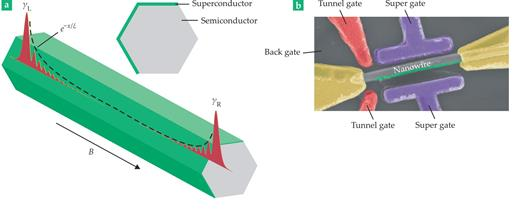
\includegraphics[width=0.75\linewidth]{img/Majorana.png}
    \caption{Nanowire mit Majorana-Quasiteilchen}
    \label{fig:Majorana}
\end{figure}

In der Abbildung ist ein Nanowire dargestellt, der durch ein Supraleiter und ein Magnetfeld in eine topologische Phase gebracht wird.
Diese Art von Partikel treten immer als Paar auf und bilden eine Art Brücke zwischen den Enden des Nanowire und besteht auf einer Vielzahl von Elektronen.
Diese Brücke wird durch die topologischen Eigenschaften der Majorana-Partikel stabilisiert und ist somit weniger anfällig gegenüber Störungen.\\


\begin{tcolorbox}[title=Kommentar,
    title filled=false,
    colback=cyan!5!white,
    colframe=cyan!75!black]
    Die Vertiefung der durch den Quanten-Hall Effekt entsteht wird nur oberflächlich behandelt. Ist jedoch essentiell für die Funktionsweise von Topologischen Quantencomputern.
\end{tcolorbox}

\textbf{Verpflechtung}\\
Braiding ist der Prozess, bei dem die Majorana-Partikel miteinander verflochten werden, um die Quantenbits zu manipulieren. 
Dies passiert auf einer zweidimensionalen Oberfläche, auf der die Majorana-Partikel miteinander verflochten werden.\\

\begin{figure}[H]
    \centering
    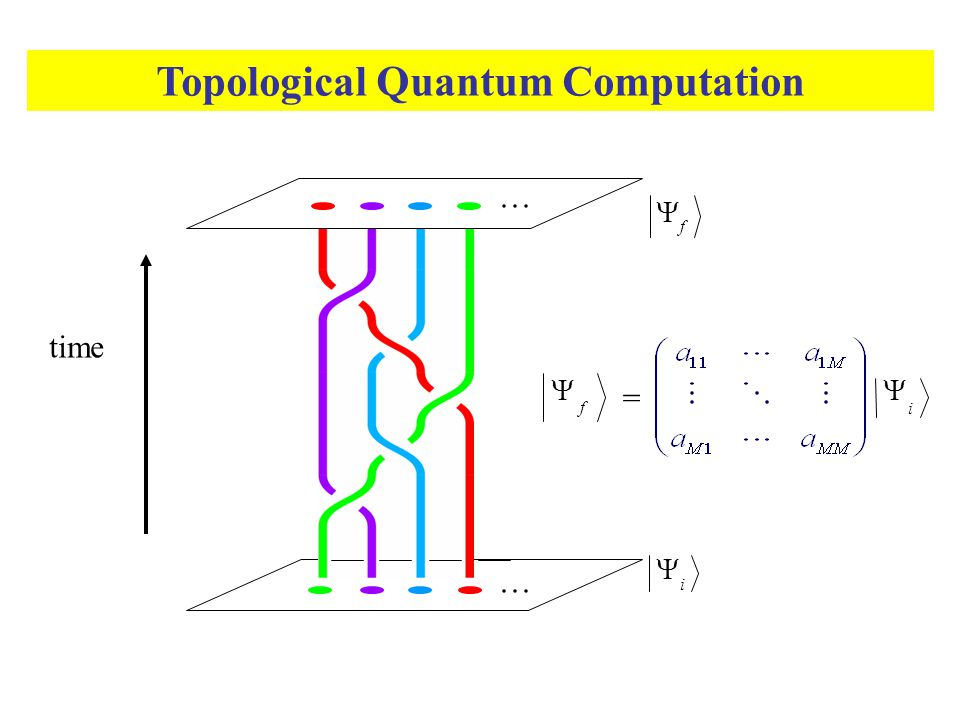
\includegraphics[width=0.75\linewidth]{img/TQC.png}
    \caption{Braiding von Majorana-Quasiteilchen}
    \label{fig:Braiding}
\end{figure}

Hierbei ist die Reihenfolge sehr wichtig, da durch diese Reihenfolge Quantenoperationen realisiert werden.
Jede Verpflechtung entspricht einer Quantenoperation und durch die Kombination von mehreren Verpflechtungen können beliebige Quantenoperationen realisiert werden.\\

Da die Informationen und Quantenoperationen in der Topologie steckt, sind sie gegenüber kleinen Fehlern in der Bewegung/Störungen unempfindlich.\\

\begin{tcolorbox}[title=Kommentar,
    title filled=false,
    colback=cyan!5!white,
    colframe=cyan!75!black]
    Die Technische Umsetzung von topologischen Quantencomputern ist deutlich komplizierter als es in diesem Abschnitt oberflächlich beschrieben ist.\\
    Bisher hat nur Google einen topologischen Quantencomputer vorgestellt, der jedoch noch nicht in der Lage ist, Quantenoperationen durchzuführen.
\end{tcolorbox}

\subsection{Quantum Error Correction}
\label{sub:quantum_error_correction}
Quantum Error Correction, oder auch QEC genannt, ist grundlegend wichtig für die funktionellen Betrieb eines Quantencomputers. Wie bereits in den vorherigen Abschnitten beschrieben,
sind Qubits sehr anfällig gegenüber Dekoheränz und Quantenrauschen.\\

\textbf{Warum ist Fehlerkorrektur notwendig}\\
Es ist unabdingbar, dass eine Fehlerkorrektur in Quantencomputern implementiert wird, da die Fehleranfälligkeit von physischen Qubits durch bessere Herstellung nur einen gewissen Grad an Fehlertoleranz aufbringen kann, welche nicht genug ist.\\

Fehler treten in Quantencomputer durch drei Hauptquellen auf.\\
1. \textbf{Dekoheränz:} Äußere Einflüsse wie Temperaturschwankungen oder elektromagnetische Felder zerstören die koheränten Eigenschaften der Qubits.\\
2. \textbf{Phasen-Flip-Fehler:} Die Phasenwinkel zwischen den Quantenzuständen werden verändert($\ket{0}\rightarrow\ket{0},\ket{1}\rightarrow-\ket{1}$).\\ 
3. \textbf{Bit-Flip-Fehler:} Die Zustände der Qubits werden verändert ($\ket{0}\rightarrow\ket{1},\ket{1}\rightarrow\ket{0}$).\\

Bei der Fehlerkorrektur von Quantencomputern ist jedoch zu beachten, dass diese nicht wie bei herkömmlichen Computern da durch das No-Cloning-Theorem keine Quanteninformationen kopiert werden können.\\

\textbf{Grundprinzip}\\
Quanten-Fehlerkorrektur verwendet \textbf{Redundanz} um Fehler zu detektieren und zu korrigieren, ohne das die eigentliche Quanteninformationen direkt ausgelesen werden.\\

Eine Art der Redundanz ist der Steane-Code, welcher auf 7 Qubits basiert. Dieser Zusammenschluss aus 7 Physischen Qubits bildet ein logisches Qubit,
welches maximal einen Fehler auf einem der 7 Qubits korrigieren kann. Treten jedoch mehrere Fehler auf, kann der Steane-Code diese nicht mehr korrigieren.\\

\begin{figure}[H]
    \centering
    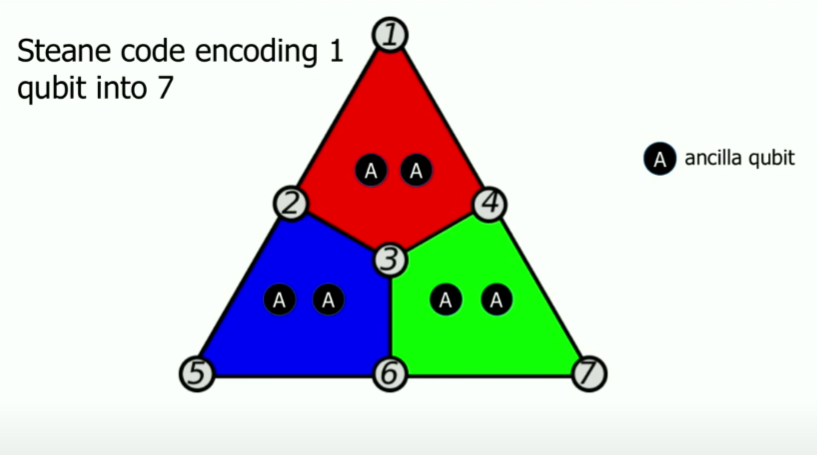
\includegraphics[width=0.75\linewidth]{img/Steane.png}
    \caption{Steane-Code}
    \label{fig:Steane}
\end{figure}

Um die Qubits zu überwachen werden zusätzliche Qubits benötigt, da das direkte Auslesen der daten Qubits den Quantenzustand zerstören würde.
Diese zusätzlichen Qubits werden als \textbf{Ancilla Qubit} bezeichnet und mit den eigentlichen Qubits verschränkt.\\

\textbf{Fehlertoleranz}\\
Diese Herangehensweise ist jedoch auch nicht perfekt. Die Ancilla Qubits sind gleichermaßen anfällig gegenüber Fehlern wie die eigentlichen Qubits.\\

\begin{figure}[H]
    \centering
    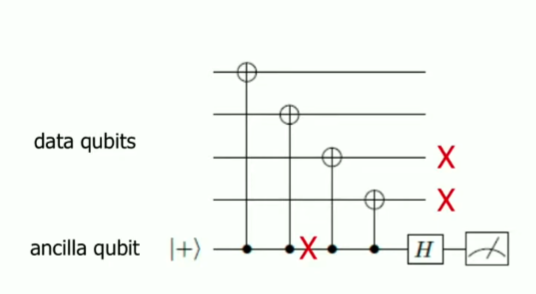
\includegraphics[width=0.75\linewidth]{img/Fehlertoleranz.png}
    \caption{Fehlertoleranz von Ancilla Qubits}
    \label{fig:Fehlertoleranz}
\end{figure}

Dieses Abbildung zeigt, wie ein einzelner Fehler in einem CNOT Gatter auf dem Ancilla Qubit Messung der Daten Qubits als Fehler kennzeichnet, obwohl diese nicht fehlerhaft sind.\\
Die Folge hieraus ist, dass die Fehlerkorrektur mit wenigen Qubits nicht ausreicht um diesen logischen Qubit vollkommen fehlerfrei zu halten.\\

Hierbei werden zwischen zwei Paritätchecks unterschieden. Ein $Z$ und $X$ Parität, welcher festlegt, ob der Fehler in den Ancilla Qubits CNOT Gattern oder den Daten Qubits aufgetreten ist.\\

\textbf{Suface Code}\\
Eine weitere Methode zur Fehlerkorrektur ist der Surface Code, welcher auf einem 2D Gitter von Qubits basiert.
Dieser Code ist in der Lage Fehler zu detektieren und zu korrigieren, solange die Fehlerdichte unter einem bestimmten Wert bleibt.\\

Die Größe des Surface Codes ist variabel und kann skaliert werden, um die Fehlerkorrektur zu verbessern.
Es gibt jedoch ein Threshold, an der die Vergößerung des Codes keine Verbesserung mehr bringt.
Durch die vorher besprochene Fehlertoleranz der Ancilla Qubits wird die Effektivität des Surface Codes gedeckelt.
Die Fehler in der Korrektur werden hierbei mehr, als wenn keine Korrektur vorgenommen wird und es würde keinen Sinn ergeben, den Surface Code weiter zu vergößern.\\

Die Nachfolgende Abbildung eines Surface Codes des Grades $d=3$ zeigt wie die Qubits in einem 2D Gitter angeordnet sind und wie die Fehlerkorrektur durchgeführt wird.
Jede Überschneidung des Gatters stellt ein physischen Qubit dar. Die Kreise in den Quadraten sind die Ancilla Qubits, welche die Fehlerkorrektur durchführen.\\

\begin{figure}[H]
    \centering
    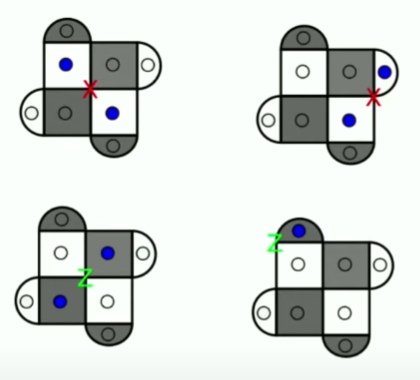
\includegraphics[width=0.6\linewidth]{img/Errors.png}
    \caption{Fehlerkorrektur durch Surface Code des Grades $d=3$}
    \label{fig:Surface-Code}
\end{figure}

Ancilla Qubits in einem weißen Feld prüfen die Qubits auf ein logisches $X$ und Ancilla Qubits in einem Schwarzen Feld prüfen die Qubits auf ein logisches $Z$.\\

Ancilla Qubits, die ein Fehler erkennen, werden als Blau markiert. Durch die Position dieser und für welche Daten Qubits diese zuständig sind wissen wir welche Qubits fehlerhaft sind.\\

\textbf{Praktische Umsetzung}\\
Am 09.12.2024 hat Google den ersten selbst korrigierenden Quantencomputer vorgestellt, der auf dem Surface Code basiert.
Der Chip namens \textbf{Willow} basiert auf 105 physischen Qubits, wobei diese auf der 7x7 Surface Code Architektur aufbaut.
Dies resultiert in 49 Qubits, die deutlich weniger anfällig gegen Fehler sind als phyische Qubits. Die restlichen Qubits werden für Parität und error Korrektur gebraucht.\\

\begin{figure}[H]
    \centering
    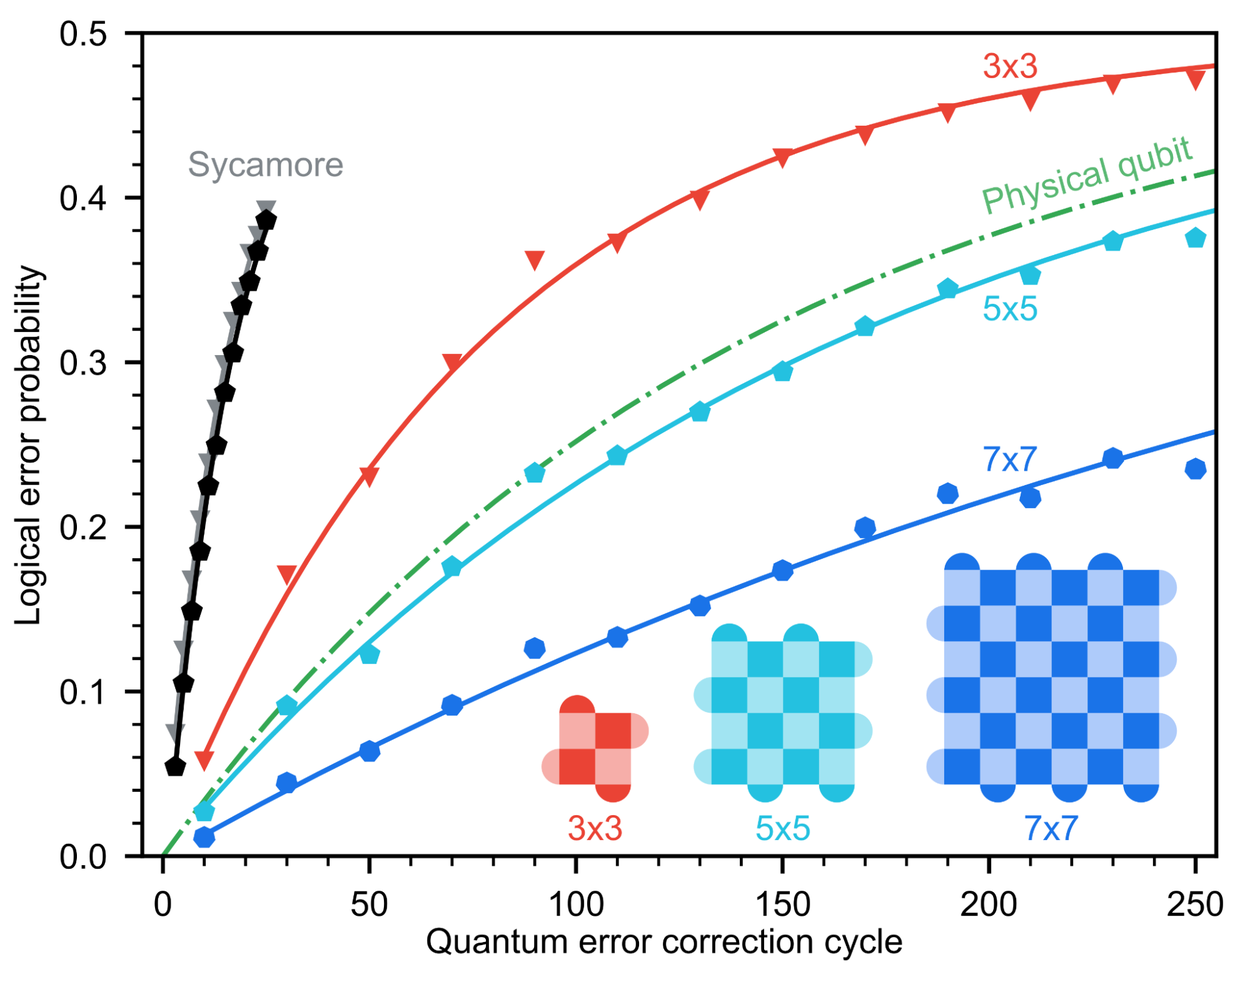
\includegraphics[width=0.7\linewidth]{img/Surface-Code-Scaling.png}
    \caption{Error Korrektur des 7x7 Surface Code}
    \label{fig:Willow}
\end{figure}

Außerdem wurde durch die Anwendung des Surface Codes die $T_1$ Zeit von $20\mu s$ auf $68\mu s\pm13\mu s$ erhöht und ermöglich hierdurch mehr Operationen pro Qubit.\\

\newpage 

\bibliographystyle{natdin}
	\bibliography{references} % expects file "references.bib"
	\addcontentsline{toc}{section}{References}
\end{document}
